\section{Question 4: Gaussian Elimination in OpenMP}

In this task we were required to parallelize the back-substitution portion of a Gaussian Elimination algorithm. 
Two versions of the algorithm were presented, each containing two for-loops. 
Additionally once parallelized, we were asked to then gauge performance of our solutions with varying scheduling types. 

  \subsection{Row-orientated algorithm}
  The algorithm to parallelize can be seen below:
  \begin{lstlisting}[language=C++]
    for (row = n-1; row >= 0; row--) 
    {
      x[row] = b[row];
      for (col = row+1; col < n; col++)
        x[row] -= A[row][col] * x[col];
      x[row] /= A[row][row];
    }
  \end{lstlisting}

  If we look at the algorithm, we see that it is not possible to parallelize the outer-loop as the inner loop relies on values generated in 
  previous iterations of the outer-loop. 
  Namely in line \textit{x[row] -= A[row][col] * x[col];}, we see \textit{x[row]} is being updated to a value which contains \textit{x[col]}. 
  Should the outer-loop be parallelized, the value of \textit{x[col]} would depend on the order at which the threads execute, thus leading to a race condition. 
  In addition, at the start of each thread, the value of \textit{x[row]} is being set to \textit{x[row] = b[row]} which would again influence the value of \textit{x[col]}.
  
  
  We can however parallelize the inner-loop safely, as we know that the value of \textit{col} is set to \textit{row+1}. And since the outer-loop is being run 
  serially counting down from \textit{numThreads}, the value of \textit{x[col]} is constant.   
  In addition, by splitting the assignment of \textit{x[row]} from the heavy calculation \textit{a[row][col] * x[col]}, we can ensure that there are no race conditions by wrapping 
  \textit{x[row]-= diff} with an \textit{\#pragma omp atomic}

  An implementation of this can be seen below:
  \begin{lstlisting}[language=C++]
    for (int row = numUnknowns - 1; row >= 0; row--)
    {
      x[row] = b[row];
      #pragma omp parallel for default(shared)
        for (int col = row + 1; col < numUnknowns; col++)
        {
          double diff = a[row][col] * x[col];
          #pragma omp atomic
          x[row] -= diff;
        }
      x[row] /= a[row][row];
    }
  \end{lstlisting}
  
  \subsection{Column-orientated algorithm}
  The algorithm to parallelize can be seen below:
  \begin{lstlisting}[language=C++]
    for (int row = 0; row < numUnknowns; row++)
      x[row] = b[row];
    for (int col = numUnknowns - 1; col >= 0; col--)
    {
      x[col] /= a[col][col];
      for (int row = 0; row < col; row++)
        x[row] -= a[row][col] * x[col];
    }
  \end{lstlisting}

  If we look at the algorithm, we see that it is not possible to parallelize the outer-loop, as both the inner-loop and outer-loop update the same variable. 
  Namely the first statement of the outer-loop \textit{x[col] /= a[col][col]} changes the value of \textit{x[col]}, the current value of \textit{x[col]} is changed during the preceding runs
  of the inner-loop. This can be seen as the inner-loop counts up from 0 towards the value of \textit{col}. Thus the value of \textit{x[col]} changes depending on the order of thread execution,
  since \textit{x[col]} is updated via division (where the order of operation does matter), this is not thread-safe and thus a data-race. 


  We can however parallelize the inner-loop safely, as we know that the value of \textit{col} is constant as \textit{row} is always less than \textit{col}, thus \textit{x[col]} is never changed.
  In addition, since \textit{row} is the inner-looper iterator, there are not data-races when updating \textit{x[row]}, thus no atomic pragma is required.

  An implementation of this can be seen below:
  \begin{lstlisting}[language=C++]
    for (int row = 0; row < numUnknowns; row++)
    x[row] = b[row];
    for (int col = numUnknowns - 1; col >= 0; col--)
    {
      x[col] /= a[col][col];
      #pragma omp parallel for default(shared)  
      for (int row = 0; row < col; row++)
          x[row] -= a[row][col] * x[col];
    }
  \end{lstlisting}

  \subsection{Results}
    When compared to the serial implementation, we have vetted that the algorithm performs as expect and produces the expected results 
    (setting \textit{u} to \textit{3} runs the application in test mode). At lower number of unknowns (3, 100 and 1000), we see an expected increase in time taken to run the program. 
    This is true for both the row and column based approaches, see figure \ref{fig:colrowlow}. 
    \begin{figure}
      \centering
      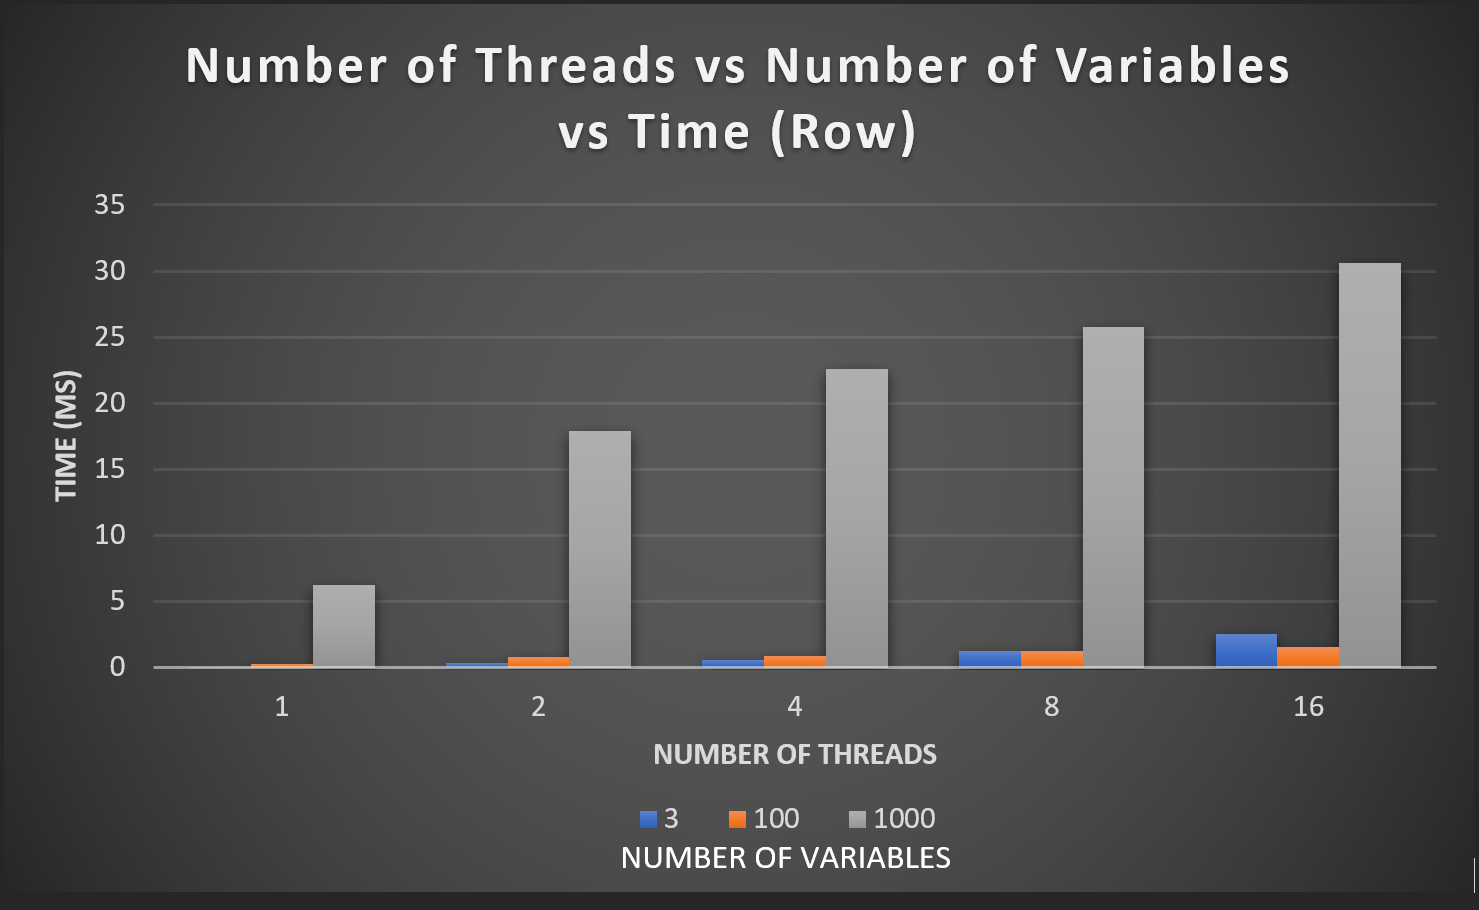
\includegraphics[width=0.49\linewidth]{Figures/rowLow.png}
      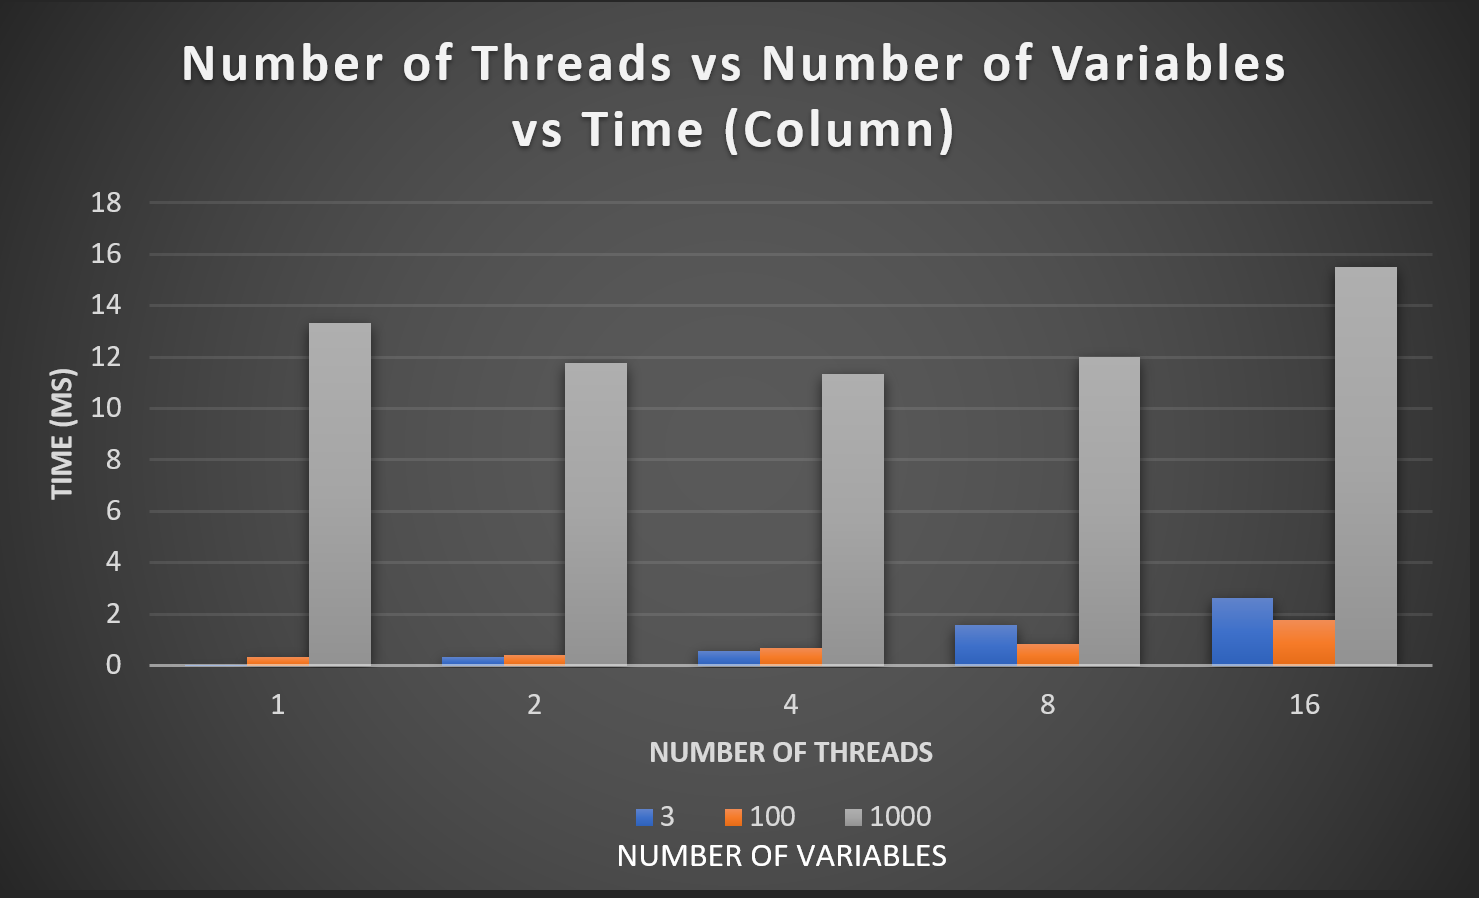
\includegraphics[width=0.49\linewidth]{Figures/colLow.png}
      \caption{Column- and Row oriented performance vs no of threads.}
      \label{fig:colrowlow}
    \end{figure}

    However, when we get to 10000 number of variables, we see that the row-based solution still increasing in time as the number of threads are added.
    This is in contrast to the column-based solution which practically halves in time as the number of threads double.
    A possible reason for this is that even though the inner-loop of the row-based solution has been parallelized, there exists a substantial calculation (namely \textit{x[row] /= a[row][row];})
    is still being done serially in addition to the atomic portion of the inner-loop. See figure \ref{fig:rowcol}.
    \begin{figure}
      \centering
      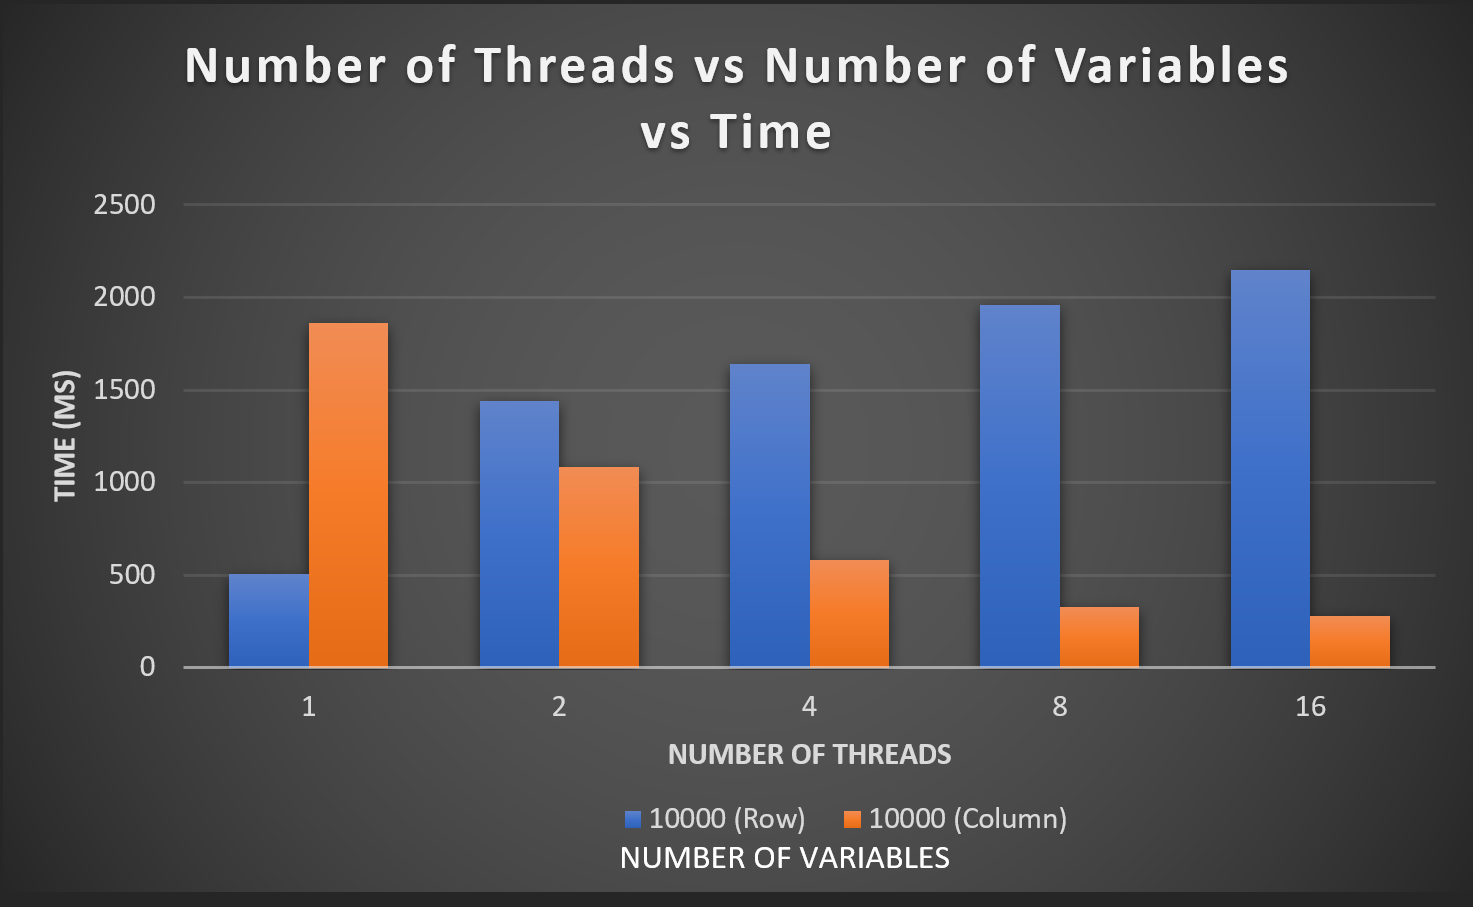
\includegraphics[width=\linewidth]{Figures/rowcol.png}
      \caption{Column- and Row oriented comparison.}
      \label{fig:rowcol}
    \end{figure}

\subsection{OpenMP Schedulers}
  This section documents our experimentation when running both the column-based solutions for 16 threads, with 42000 variables against the different OpenMP Schedulers
  \begin{lstlisting}[language=bash]
    #!/bin/bash
    set -eo pipefail

    for s in {static,dynamic,guided,auto}; do
        export OMP_SCHEDULE=$s
        filename="results_col_$OMP_SCHEDULE.txt"
        set +e
        rm $filename
        set -e
        OMP_NUM_THREADS=16 ./$PROG -u 42000 >> $filename
    done
  \end{lstlisting}
  \begin{figure}
    \centering
    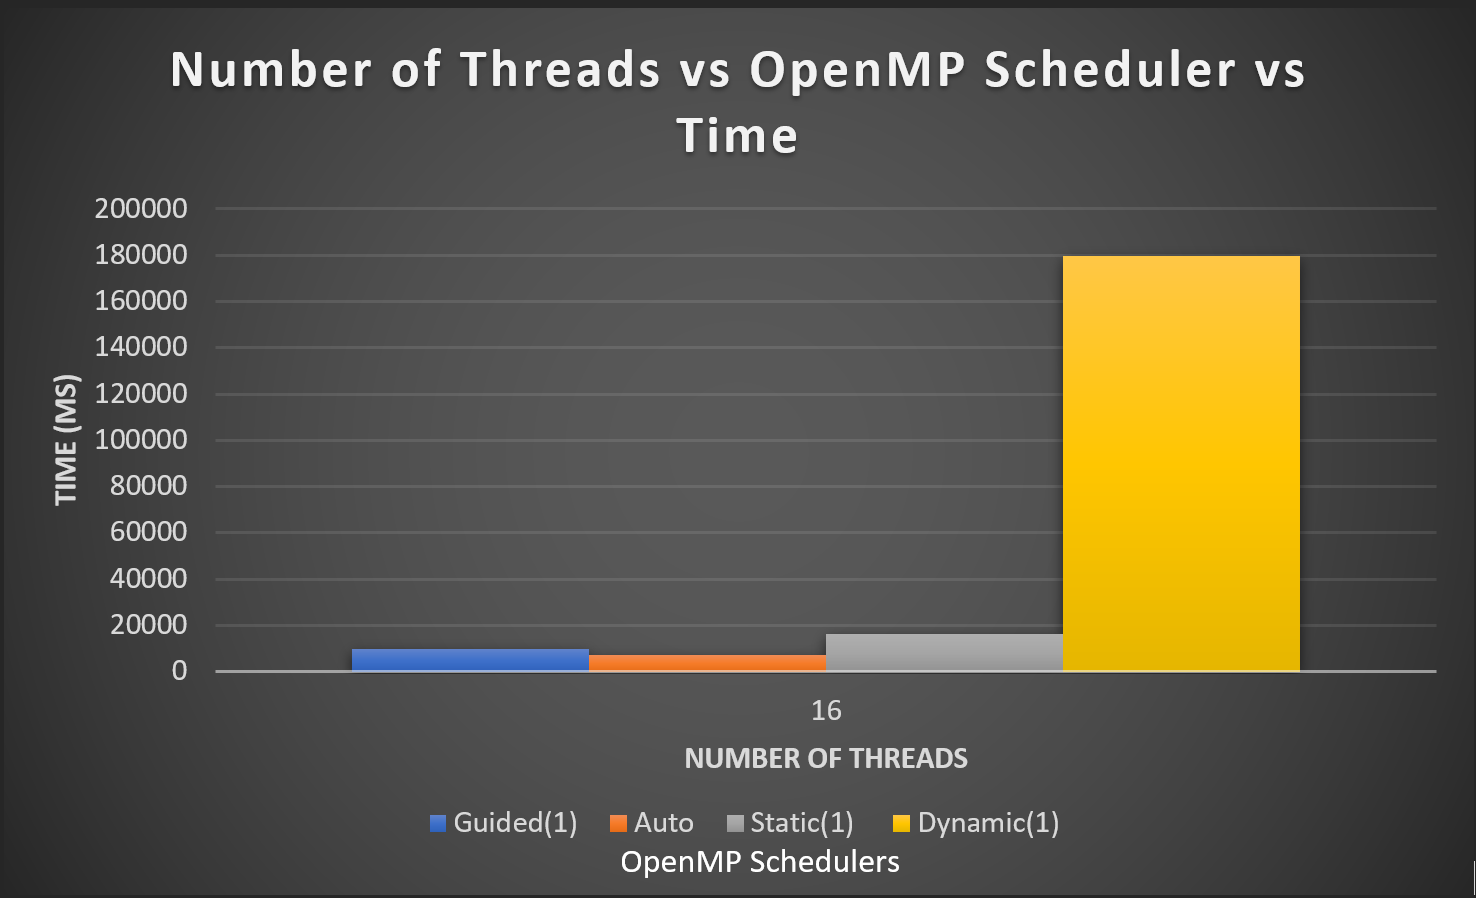
\includegraphics[width=\linewidth]{Figures/col42000.png}
    \caption{Column- and Row oriented performance vs no of threads.}
    \label{fig:col42}
  \end{figure}

  As we can see schedule type \textbf{auto} performed the best for this particular application resulting in an average increase of \textit{XXX} per thread. 
  With schedule type \textbf{dynamic} performing the worst. 
  This would track as the amount of work per iteration is vastly variable, and therefore a more generic slicing up of iteration per thread would on average perform the best.
  See figure \ref{fig:col42}.